\documentclass[10pt]{book}

%These tell TeX which packages to use.
\usepackage{array,epsfig}
\usepackage{amsmath}
\usepackage{amsfonts}
\usepackage{amssymb}
\usepackage{amsxtra}
\usepackage{amsthm}
\usepackage{mathrsfs}
\usepackage{color}
\usepackage{enumitem}
%\usepackage{mdframed}
\usepackage[most]{tcolorbox}
\usepackage{pgfplots}
\usetikzlibrary{arrows}
\pgfplotsset{compat=1.6}

\pgfplotsset{soldot/.style={color=black,only marks,mark=*}} \pgfplotsset{holdot/.style={color=black,fill=white,only marks,mark=*}}

%Here I define some theorem styles and shortcut commands for symbols I use often
\theoremstyle{definition}
\newtheorem{defn}{Definition}
\newtheorem{thm}{Theorem}
\newtheorem{cor}{Corollary}
\newtheorem*{rmk}{Remark}
\newtheorem{lem}{Lemma}
\newtheorem*{joke}{Joke}
\newtheorem{ex}{Example}
\newtheorem*{soln}{Solution}
\newtheorem{prop}{Proposition}

\newcommand{\lra}{\longrightarrow}
\newcommand{\ra}{\rightarrow}
\newcommand{\surj}{\twoheadrightarrow}
\newcommand{\graph}{\mathrm{graph}}
\newcommand{\bb}[1]{\mathbb{#1}}
\newcommand{\Z}{\bb{Z}}
\newcommand{\Q}{\bb{Q}}
\newcommand{\R}{\bb{R}}
\newcommand{\C}{\bb{C}}
\newcommand{\N}{\bb{N}}
\newcommand{\M}{\mathbf{M}}
\newcommand{\m}{\mathbf{m}}
\newcommand{\MM}{\mathscr{M}}
\newcommand{\HH}{\mathscr{H}}
\newcommand{\Om}{\Omega}
\newcommand{\Ho}{\in\HH(\Om)}
\newcommand{\bd}{\partial}
\newcommand{\del}{\partial}
\newcommand{\bardel}{\overline\partial}
\newcommand{\textdf}[1]{\textbf{\textsf{#1}}\index{#1}}
\newcommand{\img}{\mathrm{img}}
\newcommand{\ip}[2]{\left\langle{#1},{#2}\right\rangle}
\newcommand{\inter}[1]{\mathrm{int}{#1}}
\newcommand{\exter}[1]{\mathrm{ext}{#1}}
\newcommand{\cl}[1]{\mathrm{cl}{#1}}
\newcommand{\ds}{\displaystyle}
\newcommand{\vol}{\mathrm{vol}}
\newcommand{\cnt}{\mathrm{ct}}
\newcommand{\osc}{\mathrm{osc}}
\newcommand{\LL}{\mathbf{L}}
\newcommand{\UU}{\mathbf{U}}
\newcommand{\support}{\mathrm{support}}
\newcommand{\AND}{\;\wedge\;}
\newcommand{\OR}{\;\vee\;}
\newcommand{\Oset}{\varnothing}
\newcommand{\st}{\ni}
\newcommand{\wh}{\widehat}
%Pagination stuff.
\setlength{\topmargin}{-0.75in}
\setlength{\oddsidemargin}{0in}
\setlength{\evensidemargin}{0in}
\setlength{\textheight}{9.in}
\setlength{\textwidth}{6.5in}
\pagestyle{empty}
\begin{document}
\begin{flushleft}
Name:\underline{\hspace{13cm}}Date:\underline{\hspace{2cm}}
\end{flushleft}
\begin{center}
{\Large Math 1041-012 \hspace{0.5cm} Section 4.4}
\end{center}
%\vspace{0.2 cm}

\begin{tcolorbox}
\subsection*{Indeterminate Forms \& L'H\^{o}pital's Rule}
Given $f,g$ differentiable on an open interval, $g'(x)\neq 0$ (except maybe at $a$) and given a limit of the form $\displaystyle\lim_{x\rightarrow a}\frac{f(x)}{g(x)}$, where $a$ is number or $a=\pm\infty$...
\begin{itemize}
    \item If $\displaystyle\lim_{x\rightarrow a}\frac{f(x)}{g(x)}\rightarrow\frac{0}{0}$, then this is an \underline{\hspace{7cm}} of type $0/0$.
    \item If $\displaystyle\lim_{x\rightarrow a}\frac{f(x)}{g(x)}\rightarrow\frac{\infty}{\infty}$, then this is an \underline{\hspace{7cm}} of type $\infty/\infty$.
\end{itemize}
\subsection*{Rule}
If you have one of the indeterminate forms ($0/0$ or $\infty/\infty$), then
\[
\lim_{x\rightarrow a}\frac{f(x)}{g(x)}=\lim_{x\rightarrow a}\frac{f'(x)}{g'(x)}
\]
if the limit on the right side exists (or is $\pm\infty$).
\end{tcolorbox}
\textit{Remark:} The rule still holds for one sided limits.\\
\subsection*{Example 1} Compute each limit. 
\begin{enumerate}[label=(\alph*)]
    \item $\displaystyle \lim_{x\rightarrow 1}\frac{\ln x}{x-1}$\vspace{4cm}
    \item $\displaystyle \lim_{x\rightarrow \infty}\frac{e^x}{x^2}$\vspace{4cm}
    \item $\displaystyle \lim_{x\rightarrow\infty}\frac{\ln x}{\sqrt{x}}$\vspace{4cm}
    \item $\displaystyle\lim_{x\rightarrow 0}\frac{\tan x-x}{x^2}$\vspace{4cm}
    \item $\displaystyle\lim_{x\rightarrow \pi^-}\frac{\sin x}{1-\cos x}$\vspace{3cm}
    \item $\displaystyle\lim_{x\rightarrow 2^-}\frac{-3x}{2-x}$\vspace{1cm}
\end{enumerate}
\subsection*{Example 2} The graph of a function $f(x)$ and its tangent line at $x=0$ are shown. What is the value of $\displaystyle\lim_{x\rightarrow 0}\frac{f(x)}{e^x-1}$?
\begin{figure}[h!]
    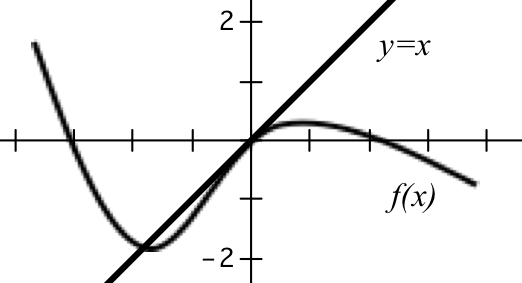
\includegraphics[width=8cm]{TantoGraph.png}
\end{figure}
\end{document}